\documentclass{article}
\usepackage[final,nonatbib]{neurips_2019}
\usepackage[utf8]{inputenc}
\usepackage[T1]{fontenc}
\usepackage{hyperref}
\usepackage{url}
\usepackage{booktabs}
\usepackage{graphicx}
\usepackage{amsmath}
\usepackage{microtype}
\usepackage{enumitem}
\usepackage{pifont}
\usepackage{xcolor}
\newcommand{\Spade}{\ding{171}}
\newcommand{\Club}{\ding{168}}
\newcommand{\Heart}{\textcolor{red!75!black}{\ding{170}}}
\newcommand{\Diam}{\textcolor{red!75!black}{\ding{169}}}
\newcommand{\file}[1]{{\small\texttt{#1}}}
\makeatletter\renewcommand{\@notice}{}\makeatother % no conference footer
\setlist{itemsep=1pt,topsep=2pt}

\title{Reading the Order Flow: Information Extraction and Leakage\\in Learned Agents for the Trading Game Figgie\\[4pt]\large Midterm report}

\author{%
  Nicholas Erup Larsen \\
  IIIS, Tsinghua University \\
  \texttt{nglsls26@mails.tsinghua.edu.cn} \\
  Student ID: 2026400695 \\
  \And
  Adriaan Van der Berg \\
  IIIS, Tsinghua University \\
  \texttt{adla26@mails.tsinghua.edu.cn} \\
  Student ID: 2026403362 \\
}

\begin{document}
\maketitle

\begin{abstract}
Figgie is a four-player card-trading game whose scoring (goal) suit is hidden.
Every published Figgie agent infers the goal suit from its own cards, yet every public trade also carries information about what the trader holds.
Our project asks how much the order flow reveals, whether reinforcement-learning (RL) agents with memory learn to read it, and whether agents that leak their own hand are easier to exploit.
At the midterm we have a shared game engine with 25 agents ported from four public sources (two of them ported decision for decision), a reproduction of the only RL agent for Figgie that matches or beats its reported numbers, and a 16{,}000-game tournament of 29 agents.
A simple model of the public trades raises goal-suit accuracy from 39\% (own hand only) to 54\% by the end of a game.
A first linear probe of the PPO agent's recurrent state finds no more about the goal suit than its card-counting input (41\% against 43\%).
With features of who traded what, untrained random-init networks of every memory architecture probe at 59--60\% on common trajectories, and every trained agent probes 6--16 points lower, so this probe measures input features rather than learned belief and cannot show that memory helps.
\end{abstract}

\section{Problem and questions}
In Figgie, 40 cards are dealt from one of 12 equally likely decks: one suit has 12 cards, one has 8 and two have 10.
The goal suit is the same-colour partner of the 12-card suit (\Spade$\leftrightarrow$\Club, \Heart$\leftrightarrow$\Diam), so it has 8 or 10 cards.
Each of the four players antes \$50 into a \$200 pot. At the end each goal card pays its holder \$10 and the rest of the pot goes to whoever holds the most goal cards.
Players trade continuously by quoting bids and asks in each suit, and every trade is public.
Because goal cards pay out, players pay more for the suit they believe is the goal, so a player who eagerly buys \Club{} probably holds many clubs and believes \Club{} is the goal.

Existing agents, such as figment's Bayesian market maker~\cite{figment}, Figgie-bot's exact inference~\cite{figgiebot} and the CS224R PPO agent~\cite{cs224r}, compute the goal-suit posterior from their own cards and at most a count of cards seen changing hands. None of them models \emph{why} an opponent trades.
Figgie is a clean test of a general question in partially observed multi-agent RL: does an agent trained only on reward learn to infer hidden state from other agents' behaviour?
The hidden state is tiny (12 decks), so the exact belief is cheap to compute and can be compared with what the network represents.
The approved proposal asks three questions:
\begin{enumerate}[label=Q\arabic*.]
  \item Revelation. How much does the public trade history reveal about the goal suit beyond a player's own hand, and how quickly? We measure the gap $\Delta_{\text{rev}}(t)$ in bits of goal-suit log-loss.
  \item Extraction. Do PPO agents with memory (none $<$ minGRU $<$ GRU $<$ transformer) learn to infer the goal suit, as tested by probing, attribution and causal interventions on their hidden state?
  \item Leakage and exploitability. Does an agent's leakage $L_a$ (how well its actions predict its hand) correlate with its exploitability $\hat\varepsilon_a$, measured by a learned PPO best response?
\end{enumerate}

\section{Work completed}

\subsection{A shared engine and verified agents}
All data is simulated in our engine (\file{figgie/engine.py}), which implements the standard rules and the CS224R discretisation: 240 ticks, one action per player per tick in a random order, 257 discrete actions, prices \$1--\$30, and every trade wipes the book.
The simulator logs the deck and all hands, so every sample carries exact ground truth.
We ported 25 agents from four public sources: the CS224R report~\cite{cs224r} (5 baselines and PPO), figment~\cite{figment} (5), Figgie-bot~\cite{figgiebot} (8) and figgie-auto~\cite{figgieauto} (7) (\file{RESULTS.md} \S1).
For figment and Figgie-bot we ran the original code inside its own simulator and fed the same observations to our port. Every decision was identical (144{,}000 of 144{,}000 and 64{,}000 of 64{,}000), and so was every goal posterior (\file{results/verify\_ports.json}).
The real-time figgie-auto bots cannot be replayed and were checked by code review only.

\subsection{Reproducing the CS224R PPO agent}
The CS224R agent~\cite{cs224r} is the only RL agent for Figgie and released no code, so we reimplemented it from the report.
A 69-dimensional observation (own hand, cash, all quotes, tick, a card-counting goal posterior and expected card values) feeds a two-layer MLP, a 128-unit GRU cell and a masked categorical actor over the 257 actions (\file{figgie/rl/policy.py}).
Training is behaviour cloning (BC) from the Bayesian baseline, then recurrent PPO~\cite{ppo} with reward shaping and prioritised fictitious self-play, 32 environments $\times$ 512 steps per update.
Version v2 up-weights lift actions 15$\times$ in cloning and adds a lift bonus in PPO. Every detail the report omits was filled with a documented guess (\file{DESIGN.md}).
After 300 updates (4.9\,M steps, one seed) PPO-v2 matches or beats every reported number of the report's Table~1 (\file{results/cs224r\_eval.json}). Against FV + Cons + MM it earns $+21.5$ \$/game and wins 52\% (reported $+8$, 54\%), and against FV + Bayes + MM $+12.7$ and 53\% (reported $+2$, 36\%), with 95\% CIs of about $\pm$4--5 (FV = FairValue, Cons = Conservative, MM = MarketMaker).


\subsection{A 29-agent tournament}
A duplicate tournament (\file{scripts/tournament.py}) draws four distinct agents per table and plays each deal under all four seat rotations, 16{,}000 games in total, with table-clustered 95\% CIs, win rate and Elo.
In a second run without uniform-random agents (\file{results/tournament\_norandom.md}) AdaptiveMM ($+22.2\pm2.4$ \$/game) is more profitable than Bayesian ($+16.1\pm2.6$) and PPO-v2 ($+15.5\pm2.2$), whose intervals do not overlap its own, with BayesianMM ($+18.4\pm2.3$) in between. No agent dominates, since PPO-v2 has the highest win rate (44.7\%) and Elo (1574).
A no-information market maker that values every card at \$8.8 sits mid-table at $+2.6$, and PotMM with its suit labels scrambled each game is last at $-48.4$, so goal-suit information is worth a great deal.

\begin{figure}[t]
  \centering
  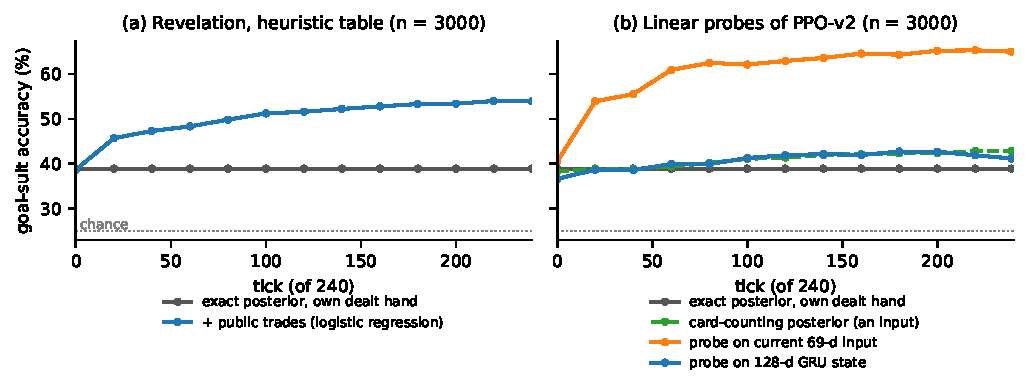
\includegraphics[width=0.75\textwidth]{midterm_results.pdf}
  \caption{Goal-suit accuracy over the game for seat 0, 3000 games, 5-fold CV. (a)~Q1: BayesianMM against Bayesian, PotMM and Fundamental. A logistic regression on the hand-only posterior plus public-trade features beats the hand-only posterior from the first trades on (\file{results/proposal\_revelation.json}). (b)~Q2: PPO-v2 at seat 0, linear probes of its current input and its GRU state (\file{results/probe\_ppo\_v2.json}). Chance is 25\%.}
  \label{fig:results}
\end{figure}

\subsection{Q1: the public trades reveal the goal suit}
We simulated 3000 games at one table (BayesianMM at seat 0 against Bayesian, PotMM and Fundamental) and every 20 ticks predicted seat 0's goal suit in two ways (\file{scripts/proposal\_figure.py}).
The baseline is the exact posterior given only seat 0's dealt hand. The order-flow model is a logistic regression that adds each opponent's net purchases per suit, the largest net position, and the number and mean price of trades per suit.
The trades help from the first 20 ticks on (Figure~\ref{fig:results}a). By tick 240 accuracy rises from 38.9\% to 54.0\% and log-loss falls from 1.88 to 1.54 bits, so $\Delta_{\text{rev}}(240)\approx 0.35$ bits (\file{results/proposal\_revelation.json}).
This is a lower bound for one table of heuristic agents, since the summaries discard the order and timing of trades.

\subsection{Q2: a first linear probe of PPO-v2}
We put PPO-v2 at seat 0 of the same table for 3000 games and recorded its input and its GRU state every 20 ticks (\file{scripts/probe\_ppo.py}). At each tick we fit 5-fold cross-validated logistic regressions on standardised features to predict the goal suit~\cite{probes}. The actor reads only the GRU state.
The result is negative for this agent (Figure~\ref{fig:results}b). The GRU state is no more informative than the card-counting posterior among its inputs, 41.2\% at tick 239 against 42.9\% (hand only 38.9\%), yet a probe of the current input reaches 65.0\% and 1.27 bits (\file{results/probe\_ppo\_v2.json}).

\subsection{Q2: PPO agents with memory of the trade flow}
\label{sec:memory}
The CS224R observation summarises the order flow only as cumulative trade counts and last prices, so it never sees \emph{who} bought what.
We add 16 features (\file{figgie/rl/features.py}): each opponent's net purchases per suit since the agent's last turn and the mean price per suit over that interval.
Accumulating them over the game requires memory.
Four policies share the CS224R encoder and differ only in the core that follows it (\file{figgie/rl/policy.py}): none, a minGRU~\cite{mingru} ($h_t=(1-z_t)\odot h_{t-1}+z_t\odot W x_t$ with gates from $x_t$ only), the CS224R GRU, and a causal two-layer, 4-head transformer~\cite{transformer} over the last 128 ticks.
The actor and the critic read only the core output, which we call the last hidden state, and a unit test checks that stepping and chunked unrolling agree across episode resets (\file{tests/test\_memory\_policies.py}).
Each run repeats the PPO-v2 recipe for 2000 updates (33\,M steps) and is then probed at the PPO-v2 table above.

Before the full table existed we committed predictions and a decision rule for it (\file{docs/PREREGISTRATION.md}).
Memory counts as helping only if a core's two-seed mean probe accuracy at tick 239 beats that of the core without memory by at least 3 points and its worse seed beats the no-memory core's better seed. A secondary criterion asks the same of profit against FV + Bayes + MM, by more than the larger per-run 95\% CI.
The only verified time is commit \texttt{b64e174} at 15:16 CET. By then minGRU s0, GRU s1 and none s1 had finished but were unseen. The transformer prediction is the only fully clean one. The minGRU prediction is clean only because nobody looked at its numbers. The GRU and no-memory predictions were written after their seed-0 results had been seen, so they are not blind.
Every comparison the file does not list is exploratory, and no setting is adopted on a single seed.

\begin{table}[h]
  \centering\scriptsize\setlength{\tabcolsep}{3pt}
  \caption{Memory agents after 2000 updates. Probe at the PPO-v2 table (3000 games, 5-fold CV), profit over 1000 games per matchup. Each cell is the mean over seeds, [min--max] over seeds, and ($\pm$ mean per-run 95\% CI). Seed 2 is additional and not part of the pre-registered test, which uses seeds 0 and 1. Transformer seed 1 resumed at update 150 on another GPU after a memory kill, with the Adam state and self-play pool reset. The hand-only posterior gives 38.9\%. Files: \file{runs/memory*/<core>\_s<seed>/\{probe,eval\}.json}, table by \file{scripts/memory\_report.py}.}
  \label{tab:memory}
    \begin{tabular}{@{}lrllll@{}}
    \toprule
    & & \multicolumn{2}{c}{Goal-suit probe accuracy (\%), tick 239} & \multicolumn{2}{c}{Profit (\$/game)} \\
    \cmidrule(lr){3-4}\cmidrule(l){5-6}
    Memory core & Seeds & Last hidden state & Current input & FV+Cons+MM & FV+Bayes+MM \\
    \midrule
    none & 3 & 53.4 [52.2--54.8] ($\pm$1.8) & 61.3 [60.3--62.6] ($\pm$1.7) & +21.8 [+20.3--+23.9] ($\pm$4.2) & +14.6 [+14.0--+15.3] ($\pm$4.3) \\
    minGRU & 3 & 56.5 [53.5--58.3] ($\pm$1.8) & 62.3 [61.6--62.8] ($\pm$1.7) & +21.5 [+21.4--+21.5] ($\pm$4.3) & +12.1 [+10.2--+15.3] ($\pm$4.3) \\
    GRU & 3 & 47.0 [46.7--47.2] ($\pm$1.8) & 63.7 [61.8--65.1] ($\pm$1.7) & +19.2 [+17.8--+20.7] ($\pm$4.2) & +11.5 [+9.0--+13.1] ($\pm$4.6) \\
    transformer & 2 & 44.8 [44.0--45.6] ($\pm$1.8) & 61.0 [60.1--62.0] ($\pm$1.7) & +9.4 [+5.8--+13.1] ($\pm$3.8) & $-$1.9 [$-$3.5--$-$0.3] ($\pm$3.8) \\
    \bottomrule
  \end{tabular}

\end{table}

The main finding is a negative control. We fed one common set of 3000 recorded games, those of the none s0 probe, through every network from a fresh state, including two untrained random-init networks per architecture (\file{runs/memory-diag/transformer\_s1/common\_probe.json}, exploratory).
On these identical inputs the current input alone probes at 60.1\%, and the random-init networks at 60.0\% (none), 60.1\% (minGRU), 60.0\% (GRU) and 59.2\% (transformer). Every trained agent is at or below that: none 53.2/54.6\%, minGRU 53.1/55.3\%, GRU 44.3/44.3\% and transformer 45.2/45.2\% for seeds 0/1.
Trained minus random-init is $-6.1$ points for none, $-5.9$ for minGRU, $-15.7$ for GRU and $-14.1$ for the transformer.
So this probe measures how much of the input's goal-suit information a network passes through, not a belief it has learned, and the comparison between memory types cannot be read as memory helping belief. The pre-registered results below stand as scored, under that reading.

Scored as sealed, on the mean of seeds 0 and 1 (\file{runs/memory/prereg/*.json}), the core without memory (54.0\%) and the GRU (47.1\%) fall inside their predicted ranges. The minGRU prediction (43--52\%) is a miss: we observed 58.0\%, and each seed (58.3\% and 57.7\%) lies above the range. The transformer prediction (48--58\%), the only fully blind one, is also a miss: we observed 44.8\% (45.6\% and 44.0\%).
The predicted order (transformer $\geq$ none $>$ GRU $\approx$ minGRU) was wrong, and the observed order is minGRU $>$ none $>$ GRU $>$ transformer.
The minGRU meets the pre-registered criterion with two seeds, confounded by policy: it beats the no-memory core by 4.0 points, and its worse seed (57.7\%) beats the better no-memory seed (54.8\%).
Each agent is probed on games it played itself, and the probe on the identical observation ranges from 60.1\% to 65.1\% across runs, so a 4-point gap lies within the spread due to policy.
We therefore do not claim that memory helps. The minGRU fails the profit criterion ($+12.8$ against $+14.9$ \$/game on seeds 0 and 1), and the GRU and the transformer meet neither criterion.
As additional evidence outside the pre-registered test, the third seed weakens the minGRU result: minGRU seed 2 reaches 53.5\%, below the better no-memory seed, and the three-seed means are 56.5\% against 53.4\%.
Both transformer seeds play a likely degenerate policy, lifting only 1--2 times per game against FV + Bayes + MM where the other cores lift 5--6 times, and at that table they have no edge: $-3.5\pm3.6$ \$/game (seed 0) and $-0.3\pm3.9$ \$/game with a 30.9\% win rate (seed 1).

Runs gru\_s0 and none\_s0 were each interrupted three times early and resumed from a checkpoint, which reset the Adam state and the self-play pool.

\section{Remaining plan}
The poster is due in the week-15 session (21--27 Dec) and the final report by 8 Jan.
\begin{itemize}
  \item Memory agents (by 21 Nov). Seeds 0--1 of all four cores and seed 2 of three are done. Then the supervised sequence model for Q1 on the full trade history and several opponent populations (by 29 Nov).
  \item Interpretability (30 Nov--13 Dec). First, replacing the probe above by a controlled one, pre-registered before it runs: the gain of each trained network over a random-init network of the same architecture on the same trajectories, and what its hidden state adds beyond the current input. Each memory core also gets a known-answer recall check, a fact shown only early in the game and probed at the end, to tell ``memory does not help'' apart from ``these agents cannot learn to use memory at this training length''. Then an extraction score $E_a$ from 0 (hand only) to 1 (as good as the Q1 model), steering along the probe direction~\cite{actadd} and ablation.
  \item Leakage and exploitability (7--20 Dec). A classifier per agent predicts its hand from its own actions, giving $L_a$ in bits. One PPO best response per agent (about 10 agents $\times$ 20\,M steps) gives $\hat\varepsilon_a$~\cite{timbers}, and we test the rank correlation of $L_a$ with $\hat\varepsilon_a$.
\end{itemize}

{\small
\begin{thebibliography}{99}\setlength{\itemsep}{0pt}\setlength{\parskip}{0pt}
\bibitem{figment} mneha05. \newblock figment: a self-play market-making arena for Figgie-style card markets. \newblock \url{https://github.com/mneha05/figment}.
\bibitem{figgiebot} revilo-25. \newblock Figgie-bot. \newblock \url{https://github.com/revilo-25/Figgie-bot}.
\bibitem{figgieauto} 0xDub. \newblock figgie-auto. \newblock \url{https://github.com/0xDub/figgie-auto}.
\bibitem{cs224r} D.~Li Yang. \newblock Reinforcement learning for Figgie: learning negotiation as a first-class skill. \newblock Stanford CS224R project report, 2026.
\bibitem{timbers} F.~Timbers et al. \newblock Approximate exploitability: learning a best response. \newblock In \emph{IJCAI}, 2022.
\bibitem{actadd} A.~M.~Turner et al. \newblock Steering language models with activation engineering. \newblock arXiv:2308.10248, 2023.
\bibitem{mingru} L.~Feng et al. \newblock Were RNNs all we needed? \newblock arXiv:2410.01201, 2024.
\bibitem{transformer} A.~Vaswani et al. \newblock Attention is all you need. \newblock In \emph{NeurIPS}, 2017.
\bibitem{ppo} J.~Schulman et al. \newblock Proximal policy optimization algorithms. \newblock arXiv:1707.06347, 2017.
\bibitem{probes} G.~Alain and Y.~Bengio. \newblock Understanding intermediate layers using linear classifier probes. \newblock arXiv:1610.01644, 2016.
\end{thebibliography}
}

\end{document}
